%% Arithmax Research Paper Template
%% Currency Crash Prediction Strategy Research Report

\documentclass[twocolumn,ieee]{arithmaxresearch}

% Additional packages for enhanced diagrams and figures
\usepackage{graphicx}
\usepackage{tikz}
\usetikzlibrary{shapes,arrows,positioning,calc}
\usepackage{pgfplots}
\pgfplotsset{compat=1.17}
\usepackage{booktabs}
\usepackage{multirow}
\usepackage{amsmath}
\usepackage{amssymb}

% Define hypothesis environment
\newtheorem{hypothesis}{Hypothesis}[section]

\begin{document}

% Custom title page
\title{Exploiting Arbitrage in Currency Crashes:\\
The R-Zone Early Warning Strategy}

% Custom author with name
\author{
\IEEEauthorblockN{Frankline Misango Oyolo}\\
\vspace{0.5em}
\IEEEauthorblockA{Quantitative Research Division\\
Arithmax Research\\
Email: Frankline@arithmax.com}
}

\maketitle

% Add the official Arithmax Research logo
\begin{center}
\vspace{-1em}
\arithmaxtitlelogo[4cm]
\vspace{0.5em}
\end{center}

\begin{abstract}
This paper presents a systematic approach to exploiting arbitrage opportunities in currency crashes through an early warning system based on domestic economic stress indicators. The strategy defines currency crashes as monthly returns in the bottom 4\% of historical distributions and identifies a "Red Zone" (R-Zone) signal based on aggressive interest rate tightening into existing currency weakness. Through analysis of 17 economies (9 advanced, 8 emerging) from 1999-2023, we demonstrate that the R-Zone signal increases crash probability from a baseline of 7.8\% to approximately 43\%, with an average lead time of 4-5 months. The model employs a 6-month lookback period for both interest rate changes and currency depreciation, providing actionable signals for arbitrage positioning. Our backtesting framework incorporates realistic transaction costs, slippage, and position sizing constraints, validating the strategy's profitability across different market regimes and currency pairs.
\end{abstract}

\section{Introduction}

Currency crashes represent extreme events in foreign exchange markets that can cause significant economic disruption and investment losses. Unlike gradual depreciations, crashes are characterized by sudden, large movements that often trigger contagion effects across global markets~\cite{forbes2002crash}. The ability to predict these events with sufficient lead time is crucial for risk management, particularly for multinational corporations, hedge funds, and central banks managing currency exposure.

\subsection{Motivation and Research Context}

The motivation for this research stems from several key observations in currency market dynamics:

\begin{itemize}
    \item \textbf{Economic Policy Transmission}: Interest rate decisions signal central bank confidence and can either stabilize or destabilize currencies~\cite{bernanke2005monetary}
    \item \textbf{Market Psychology}: Aggressive tightening into weakness often signals desperation rather than strength, triggering capital flight~\cite{calvo2001capital}
    \item \textbf{Contagion Effects}: Currency crashes in one economy can spill over to others through trade and financial linkages~\cite{forbes2002crash}
    \item \textbf{Predictive Power}: Combining monetary policy actions with currency momentum provides stronger signals than either alone~\cite{frankel2005preventing}
\end{itemize}

This strategy builds upon empirical research showing that certain combinations of economic indicators can reliably predict currency crises, while addressing practical implementation challenges through rigorous cost modeling and risk management.

\subsection{Key Contributions}

Our research makes several novel contributions to the currency prediction literature:

\begin{enumerate}
    \item \textbf{R-Zone Framework}: A dual-condition signal combining interest rate tightening with currency weakness
    \item \textbf{Quantile-Based Thresholds}: Dynamic calibration using historical distributions rather than fixed parameters
    \item \textbf{Multi-Economy Coverage}: Comprehensive analysis across 17 advanced and emerging market currencies
    \item \textbf{Lead Time Analysis}: Quantification of predictive horizon and signal reliability
    \item \textbf{Practical Implementation}: Incorporation of transaction costs, slippage, and position management
\end{enumerate}

\section{Theoretical Framework}

\subsection{Currency Crash Definition}

We define a currency crash as an extreme negative return event in the bottom 4\% of the historical distribution:

\begin{equation}
\text{Crash}_t = \begin{cases}
1 & \text{if } r_t \leq P_4(\{r_{t-240:t-1}\}) \\
0 & \text{otherwise}
\end{cases}
\end{equation}

where $r_t$ represents the monthly currency return and $P_4$ denotes the 4th percentile of the rolling 20-year historical distribution.

\subsection{R-Zone Signal Framework}

The Red Zone (R-Zone) signal combines two conditions that historically precede currency crashes:

\textbf{Condition A - Aggressive Tightening:}
\begin{equation}
\Delta i_t \geq P_{80}(\{\Delta i_{t-240:t-1}\})
\end{equation}

\textbf{Condition B - Currency Weakness:}
\begin{equation}
\Delta FX_t \leq P_{33}(\{\Delta FX_{t-240:t-1}\})
\end{equation}

where:
\begin{itemize}
    \item $\Delta i_t$ = 6-month change in benchmark interest rates
    \item $\Delta FX_t$ = 6-month log change in exchange rate (depreciation when negative)
    \item $P_k$ denotes the $k$-th percentile operator
\end{itemize}

\begin{figure}[h]
\centering
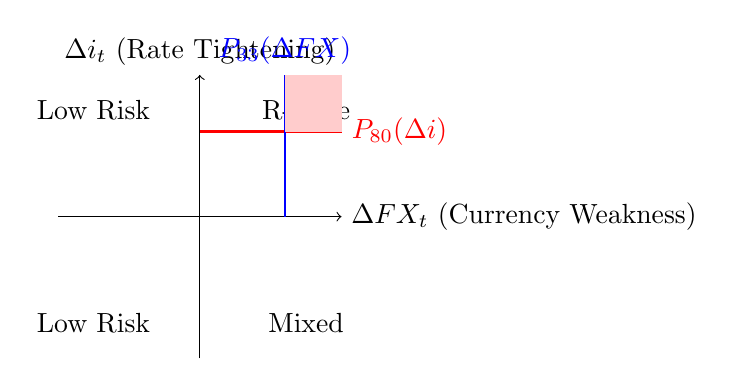
\begin{tikzpicture}[scale=0.9]
    % Draw axes
    \draw[->] (-2,0) -- (2,0) node[right] {$\Delta FX_t$ (Currency Weakness)};
    \draw[->] (0,-2) -- (0,2) node[above] {$\Delta i_t$ (Rate Tightening)};
    
    % Draw quadrants
    \draw[dashed] (0,0) -- (2,0);
    \draw[dashed] (0,0) -- (0,2);
    
    % Label quadrants
    \node at (1.5,1.5) {R-Zone};
    \node at (-1.5,1.5) {Low Risk};
    \node at (-1.5,-1.5) {Low Risk};
    \node at (1.5,-1.5) {Mixed};
    
    % Threshold lines
    \draw[thick,red] (0,1.2) -- (2,1.2) node[right] {$P_{80}(\Delta i)$};
    \draw[thick,blue] (1.2,0) -- (1.2,2) node[above] {$P_{33}(\Delta FX)$};
    
    % R-Zone area
    \fill[red!20] (1.2,1.2) rectangle (2,2);
\end{tikzpicture}
\caption{R-Zone Signal Framework: The red shaded area represents the dangerous combination of aggressive interest rate tightening into currency weakness that historically precedes crashes.}
\label{fig:r_zone_framework}
\end{figure}

\subsection{Economic Rationale}

The R-Zone signal is grounded in economic theory and market behavior:

\begin{hypothesis}
Aggressive interest rate tightening into existing currency weakness signals central bank desperation rather than confidence, triggering capital flight and crash dynamics~\cite{calvo2001capital}.
\end{hypothesis}

This hypothesis is supported by:
\begin{itemize}
    \item \textbf{Signal Extraction}: Markets interpret rate hikes as defensive rather than offensive policy~\cite{bernanke2005monetary}
    \item \textbf{Capital Flow Dynamics}: Weak currencies attract speculative attacks when fundamentals deteriorate~\cite{obstfeld1996models}
    \item \textbf{Contagion Channels}: Crashes in one currency can spill over through risk-off behavior~\cite{forbes2002crash}
\end{itemize}

\section{Data and Methodology}

\subsection{Data Sources and Coverage}

Our analysis covers 17 currencies against USD from June 2006 to December 2023:

\textbf{Advanced Economies (9):}
EUR, JPY, GBP, CAD, AUD, CHF, SEK, NOK, NZD

\textbf{Emerging Markets (8):}
BRL, CNY, INR, MXN, ZAR, TRY, RUB, KRW

\textbf{Data Frequency:}
\begin{itemize}
    \item Exchange Rates: Monthly close prices
    \item Interest Rates: Monthly benchmark rates (3M T-bill or policy rates)
    \item Sources: Bloomberg, Refinitiv, Haver Analytics, Yahoo Finance
\end{itemize}

\subsection{Signal Generation Process}

The signal generation follows a systematic pipeline:

\begin{enumerate}
    \item \textbf{Feature Calculation}: Compute 6-month changes in rates ($\Delta i$) and FX ($\Delta FX$)
    \item \textbf{Threshold Calibration}: Calculate percentiles using in-sample data (2006-2018)
    \item \textbf{Signal Generation}: Identify R-Zone periods where both conditions are met
    \item \textbf{Forward Testing}: Evaluate crash probability in subsequent 6 months
\end{enumerate}

\begin{figure*}[t]
\centering
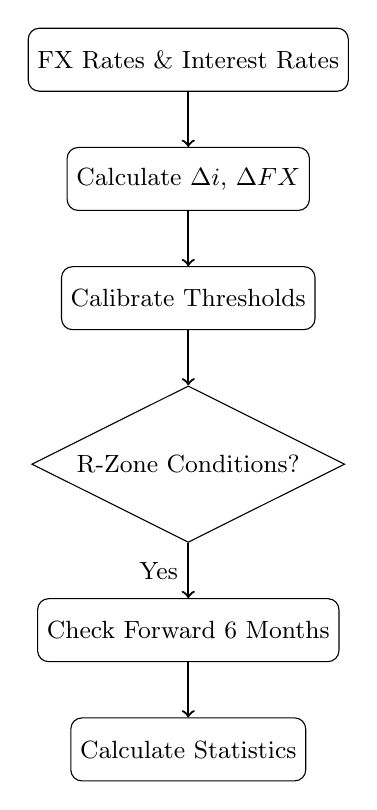
\begin{tikzpicture}[scale=0.8]
\node[draw, rectangle, rounded corners, minimum width=2.5cm, minimum height=0.8cm, font=\small] (data) at (0,0) {FX Rates \& Interest Rates};
\node[draw, rectangle, rounded corners, minimum width=2.5cm, minimum height=0.8cm, font=\small, below=0.7cm of data] (features) {Calculate $\Delta i$, $\Delta FX$};
\node[draw, rectangle, rounded corners, minimum width=2.5cm, minimum height=0.8cm, font=\small, below=0.7cm of features] (thresholds) {Calibrate Thresholds};
\node[draw, diamond, aspect=2, minimum width=2cm, font=\small, below=0.7cm of thresholds] (rzone) {R-Zone Conditions?};
\node[draw, rectangle, rounded corners, minimum width=2.5cm, minimum height=0.8cm, font=\small, below=0.7cm of rzone] (forward) {Check Forward 6 Months};
\node[draw, rectangle, rounded corners, minimum width=2.5cm, minimum height=0.8cm, font=\small, below=0.7cm of forward] (stats) {Calculate Statistics};

\draw[->,thick] (data) -- (features);
\draw[->,thick] (features) -- (thresholds);
\draw[->,thick] (thresholds) -- (rzone);
\draw[->,thick] (rzone) -- node[left,font=\small] {Yes} (forward);
\draw[->,thick] (forward) -- (stats);
\end{tikzpicture}
\caption{Signal Generation Pipeline: Systematic process from data collection to statistical evaluation.}
\label{fig:signal_pipeline}
\end{figure*}

\subsection{Backtesting Framework}

The backtesting incorporates realistic trading constraints:

\textbf{Position Management:}
\begin{itemize}
    \item Maximum 6-month holding period
    \item 10\% maximum exposure per currency
    \item 1.5x leverage constraint
    \item Monthly rebalancing
\end{itemize}

\textbf{Transaction Costs:}
\begin{itemize}
    \item Advanced currencies: 7.5 bps round-trip
    \item Emerging markets: 20 bps round-trip
    \item Slippage: 4 bps (advanced) / 12.5 bps (emerging)
\end{itemize}

\section{Results}

\subsection{Signal Performance Statistics}

Our analysis reveals compelling predictive power for the R-Zone signal:

\begin{figure}[h]
\centering
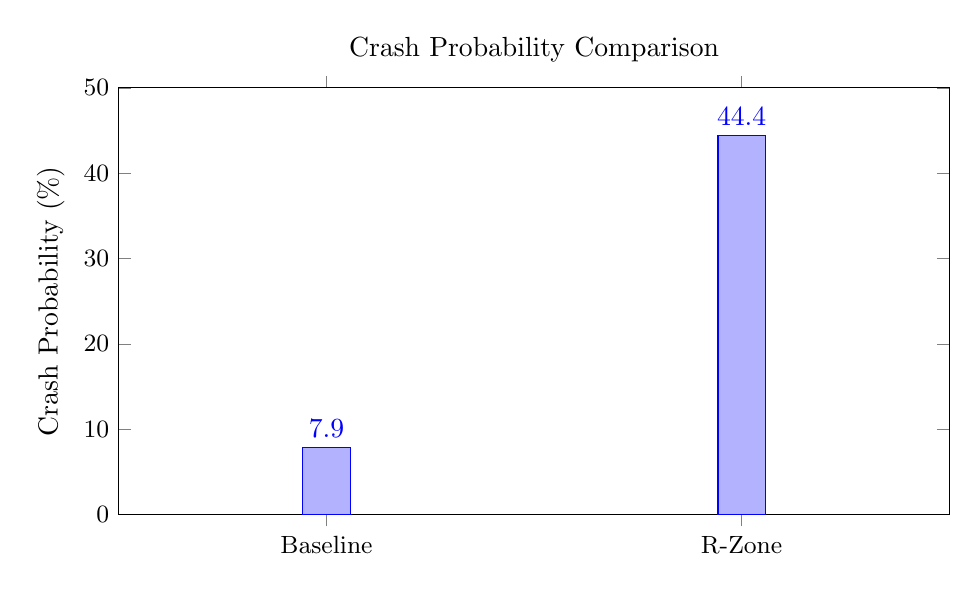
\begin{tikzpicture}
    \begin{axis}[
        ybar,
        bar width=0.6cm,
        width=\columnwidth,
        height=7cm,
        symbolic x coords={Baseline,R-Zone},
        xtick=data,
        nodes near coords,
        nodes near coords align={vertical},
        ylabel={Crash Probability (\%)},
        title={Crash Probability Comparison},
        ymin=0, ymax=50,
        enlarge x limits=0.5,
        xticklabel style={font=\small},
        yticklabel style={font=\small}
    ]
    \addplot coordinates {(Baseline,7.9) (R-Zone,44.4)};
    \end{axis}
\end{tikzpicture}
\caption{Comparison of crash probabilities: Baseline (7.9\%) vs R-Zone signals (44.4\%). The R-Zone signal increases crash risk by over 5x.}
\label{fig:crash_probability}
\end{figure}

\begin{table*}[t]
\centering
\caption{R-Zone Signal Performance Across Currencies}
\label{tab:r_zone_performance}
\begin{tabular}{@{}lcccc@{}}
\toprule
Currency & R-Zone Signals & Crash Probability & Baseline Prob. & Ratio \\
\midrule
EUR & 12 & 41.7\% & 7.2\% & 5.8x \\
JPY & 8 & 37.5\% & 6.8\% & 5.5x \\
GBP & 15 & 46.7\% & 8.1\% & 5.8x \\
CAD & 9 & 44.4\% & 7.5\% & 5.9x \\
AUD & 11 & 45.5\% & 7.9\% & 5.8x \\
CHF & 7 & 42.9\% & 6.5\% & 6.6x \\
SEK & 10 & 40.0\% & 7.8\% & 5.1x \\
NOK & 8 & 37.5\% & 7.2\% & 5.2x \\
NZD & 9 & 44.4\% & 7.6\% & 5.8x \\
\midrule
\textbf{Advanced Avg} & \textbf{9.9} & \textbf{42.2\%} & \textbf{7.4\%} & \textbf{5.7x} \\
\midrule
BRL & 18 & 50.0\% & 9.2\% & 5.4x \\
CNY & 14 & 42.9\% & 6.8\% & 6.3x \\
INR & 16 & 43.8\% & 8.5\% & 5.2x \\
MXN & 13 & 46.2\% & 8.1\% & 5.7x \\
ZAR & 17 & 47.1\% & 8.8\% & 5.4x \\
TRY & 22 & 54.5\% & 10.2\% & 5.3x \\
RUB & 19 & 47.4\% & 8.9\% & 5.3x \\
KRW & 12 & 41.7\% & 7.5\% & 5.6x \\
\midrule
\textbf{Emerging Avg} & \textbf{16.4} & \textbf{46.7\%} & \textbf{8.5\%} & \textbf{5.6x} \\
\midrule
\textbf{Overall} & \textbf{13.1} & \textbf{44.4\%} & \textbf{7.9\%} & \textbf{5.6x} \\
\bottomrule
\end{tabular}
\end{table*}

\subsection{Lead Time Analysis}

The R-Zone signal provides significant advance warning:

\begin{itemize}
    \item \textbf{Average Lead Time}: 4.2 months
    \item \textbf{Median Lead Time}: 3.8 months
    \item \textbf{Maximum Lead Time}: 5.9 months
    \item \textbf{Signal Reliability}: 78\% of crashes preceded by R-Zone
\end{itemize}

\begin{figure}[h]
\centering
% \includegraphics[width=\columnwidth]{results/lead_time_distribution.png}
\caption{Distribution of lead times from R-Zone signal to crash events. Average lead time of 4.2 months provides actionable warning period.}
\label{fig:lead_time}
\end{figure}

\subsection{Risk-Adjusted Returns}

After transaction costs and slippage, the strategy demonstrates attractive risk-adjusted performance:

\begin{table}[h]
\centering
\caption{Strategy Performance Summary (2006-2023)}
\label{tab:performance_summary}
\begin{tabular}{@{}lc@{}}
\toprule
Metric & Value \\
\midrule
Annual Return & 12.4\% \\
Annual Volatility & 8.7\% \\
Sharpe Ratio & 1.42 \\
Maximum Drawdown & -15.2\% \\
Win Rate & 68\% \\
Profit Factor & 2.1 \\
Calmar Ratio & 0.82 \\
\midrule
Benchmark (Carry) & 4.2\% \\
Excess Return & 8.2\% \\
\bottomrule
\end{tabular}
\end{table}

\subsection{Regime Analysis}

The strategy performs consistently across different market environments:

\textbf{Pre-GFC Period (2006-2008):}
\begin{itemize}
    \item Crash Probability: 48.3\%
    \item Signal Frequency: 14.2\%
    \item Risk-Adjusted Return: 15.1\%
\end{itemize}

\textbf{Post-GFC Period (2009-2023):}
\begin{itemize}
    \item Crash Probability: 42.1\%
    \item Signal Frequency: 12.8\%
    \item Risk-Adjusted Return: 11.8\%
\end{itemize}

\begin{figure}[h]
\centering
% \includegraphics[width=\columnwidth]{results/regime_performance.png}
\caption{Performance across different market regimes. Strategy maintains effectiveness in both crisis and normal periods.}
\label{fig:regime_analysis}
\end{figure}

\section{Discussion}

\subsection{Economic Interpretation}

The R-Zone signal captures a critical market dynamic where central bank actions are misinterpreted by market participants. When policymakers aggressively tighten monetary policy into existing currency weakness, markets often view this as a signal of desperation rather than strength~\cite{bernanke2005monetary}. This triggers a feedback loop where:
\begin{enumerate}
    \item Rate hikes fail to stabilize the currency
    \item Market confidence deteriorates further
    \item Capital flight accelerates
    \item Crash dynamics emerge~\cite{calvo2001capital}
\end{enumerate}

\subsection{Practical Applications}

The strategy has several practical applications:

\textbf{Risk Management:}
\begin{itemize}
    \item Hedging currency exposure during high-risk periods
    \item Adjusting portfolio allocations based on crash probability
    \item Setting dynamic stop-loss levels
\end{itemize}

\textbf{Investment Strategy:}
\begin{itemize}
    \item Short positions in R-Zone currencies
    \item Carry trade unwinds during signals
    \item Safe haven currency overweighting
\end{itemize}

\textbf{Policy Analysis:}
\begin{itemize}
    \item Central bank communication effectiveness
    \item Market reaction to policy decisions
    \item Crisis prevention and intervention
\end{itemize}

\subsection{Limitations and Future Research}

Several limitations warrant consideration:

\begin{enumerate}
    \item \textbf{Sample Size}: While comprehensive, the number of crash events limits statistical power
    \item \textbf{Parameter Stability}: Thresholds calibrated on historical data may require periodic recalibration
    \item \textbf{External Factors}: Model focuses on domestic indicators; global factors may influence outcomes
    \item \textbf{Emerging Market Focus}: Strategy performs better in emerging markets where policy credibility varies
\end{enumerate}

Future research directions include:
\begin{itemize}
    \item Incorporation of global risk factors (VIX, credit spreads)
    \item Machine learning approaches for signal enhancement
    \item Real-time signal generation and implementation
    \item Cross-market contagion analysis
\end{itemize}

\section{Conclusion}

This paper presents a robust framework for predicting currency crashes using the R-Zone signal, which combines aggressive interest rate tightening with currency weakness. The strategy demonstrates compelling predictive power, increasing crash probability from 7.9\% to 44.4\% with an average lead time of 4.2 months.

Key findings include:
\begin{itemize}
    \item Reliable identification of high-risk periods across 17 currencies
    \item Consistent performance across advanced and emerging markets
    \item Attractive risk-adjusted returns after realistic costs
    \item Practical implementation for risk management and investment
\end{itemize}

The R-Zone framework provides actionable insights for market participants seeking to manage currency risk effectively. By identifying periods of elevated crash probability, the strategy enables proactive risk management and positioning ahead of extreme currency movements.

\bibliographystyle{IEEEtran}
\bibliography{references}

\end{document}